\renewcommand{\SourceFile}{4-arborescences/src/4-2.ml}

\section{Arbre bicolore}

\Q
Un arbre binaire étiqueté est défini par une racine, des nœuds et des feuilles. Un nœud est défini par un père, un fils gauche, un fils droit, un étiquette (entier positif) et une couleur (noir ou rouge). La racine est un nœud sans père et une feuille est un nœud vide (autrement dit, fils vide d'un nœud interne).
\medskip

Expliquer quelle structure de donnée utiliser pour représenter un arbre binaire étiqueté en OCaml.

\Q
Un arbre binaire est de recherche (ABR) si chaque nœud est tel que : tout nœud de sa sous arborescence droite ne contient que des valeurs d'étiquettes supérieures et tout nœud de sa sous-arborescence gauche des valeurs d'étiquettes inférieures.
\medskip

Donne une fonction permettant d'insérer une nouvelle valeur en conservant la structure d'ABR.

\Q
Un arbre bicolore est un arbre binaire de recherche qui vérifie les propriétés suivantes : chaque nœud est soit noir, soit rouge, chaque feuille est considérée comme noire, si un nœud est rouge alors ses deux fils sont noirs et tous les chemins d'un nœud $(x)$ à une feuille de sa descendance contiennent le même nombre $\textbf{np}(x)$ de nœuds noirs (non-compris le nœud lui-même). Ce nombre est appelé la \textbf{noire-profondeur} du nœud.
\medskip

Nous définissons la \textbf{noire-profondeur d'un arbre bicolore} comme étant la noire-profondeur de sa racine.
\medskip

Montrer que la profondeur (longueur de la plus longue branche, \textit{racine $\rightarrow$ feuille}) d'un arbre bicolore composé de $n$ nœuds internes (i.e qui ne sont pas des feuilles) est d'au plus $2\log_2(n+1)$.

\Q
Nous désirons effectuer les rotations suivantes, où $T$ représente l'arbre :
\bigskip

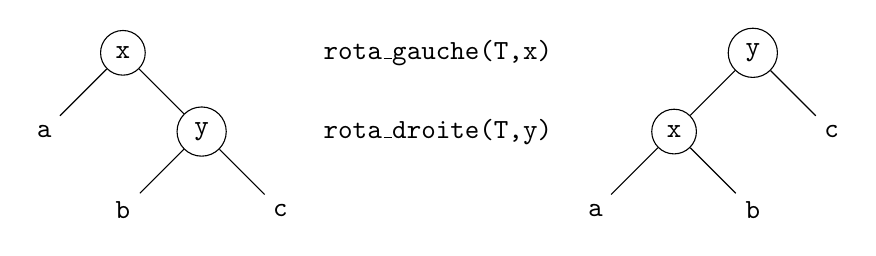
\begin{tikzpicture}[sibling distance=2cm, level distance=1cm, every node/.style={font=\ttfamily}]
    \node[draw, circle] {x}
    child {node {a}}
    child {node[draw, circle] {y}
        child {node {b}}
        child {node {c}}
    };

    \node[draw, circle, xshift=8cm] {y}
    child {node[draw, circle] {x}
        child {node {a}}
        child {node {b}}
    }
    child {node {c}};

    \node at (4,0) {$\underrightarrow{\texttt{rota\_gauche(T,x)}}$};
    \node at (4,-1) {$\underleftarrow{\texttt{rota\_droite(T,y)}}$};

\end{tikzpicture}
\bigskip

Écrire la fonction \texttt{rota\_gauche}.
\smallskip

Montrer que cette fonction préserve la structure d'arbre binaire de recherche. En est-il de même de la structure d'arbre rouge-noir ?

\Q
Comment insérer un nouvel élément dans un arbre bicolore en conservant sa structure ?

\Corrige

\Q
On représente un arbre bicolore avec le type récursif suivant :

\lstinputlisting[linerange={1-2}]{\SourceFile}

\Q
Pour insérer un nouvel élément dans un arbre binaire de recherche en conservant la propriété fondamentale des ABR, nous parcourons l'arborescence en partant de la racine avec comme critère de choix pour le nœud suivant le fils droit si l'étiquette du nouvel élément est plus grande que celle du nœud courant et le fils gauche sinon.
\medskip

En OCaml, on peut écrire :

\lstinputlisting[linerange={4-8}]{\SourceFile}

\Q
L'arbre bicolore minimal pour une noire-profondeur $np$ donnée n'est composé que de nœuds noirs. Comme chaque branche partant de la racine a exactement $np$ nœuds noirs, nous avons un arbre complet équilibré de profondeur $np$. Chaque niveau $i$ de cet arbre avant tout binaire contient $2^i$ nœuds.
\medskip

Ainsi, un arbre bicolore de noire-profondeur $np$ est composé d'au moins $2^{np}-1$ nœuds noirs.
\medskip

Si $n$ est le nombre de nœuds d'un arbre bicolore de noire-profondeur $np$, nous avons
\[
    n \geq 2^{np}-1
\]
autrement dit,
\[
    \log_2(n+1) \geq np
\]

Si l'on tient compte du fait que, sur une branche, au plus un nœud sur deux est rouge, la profondeur d'un arbre bicolore de noire-profondeur $np$ est au plus $2np$ c'est à dire d'au plus $2\log_2(n+1)$.

\Q
Pour alléger les fonctions et puisque la coloration n'apporte rien ici, on définit un type d'arbre binaire sans couleurs :

\lstinputlisting[linerange={15-15}]{\SourceFile}

On propose les fonctions de rotations gauche et droite autour de la racine de \texttt{t} (la transformation n'est pas effectuée si elle est impossible) :

\lstinputlisting[linerange={17-23}]{\SourceFile}

Si l'on souhaite effectuer une rotation autour d'un nœud en particulier, il suffit de descendre jusqu'à celui-ci de manière récursive puis de le remplacer, similairement à ce qui est fait pour l'insertion :

\lstinputlisting[linerange={25-29}]{\SourceFile}

La fonction \texttt{rotate\_node\_right} s'écrit de manière analogue.
\medskip

La structure d'arbre binaire de recherche est conservée : $x$ et $y$ sont du même côté par rapport au père de $x$ et les étiquettes de la sous-arborescence gauche de $y$ sont supérieures à celle de $x$ et inférieures à celle de $y$, elle peut devenir la sous-arborescence droite de $x$ sans que l'arbre ne perde sa propriété d'arbre binaire de recherche.
\newpage

En revanche, la propriété d'arbre bicolore n'est pas forcément conservée. Si nous appliquons l'algorithme précédent à l'arbre ci-dessous où les nœuds noirs sont colorés en noir et les nœuds rouges sont représentés en blanc :
\medskip

\tikzstyle{nil}=[fill=black, label={[yshift=4pt, xshift=-2pt]south:nil}, inner sep=0pt]
\tikzstyle{short}=[level distance=7mm, sibling distance=1cm]
\tikzstyle{black}=[fill=black, text=white]
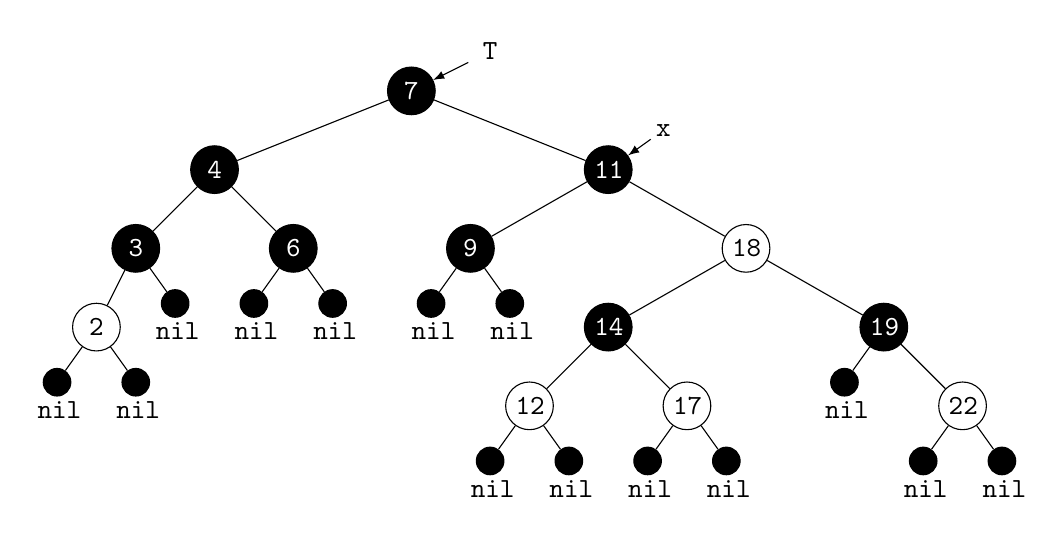
\begin{tikzpicture}
    [edge from parent/.style={draw,-},
    every node/.style={
        text width=1em,
        align=center,
        font=\ttfamily,
        draw,
        circle,
        inner sep=2pt,
        minimum size=8pt},
    level distance=1cm,
    level 1/.style={sibling distance=5cm},
    level 2/.style={sibling distance=2cm},
    level 3/.style={sibling distance=1cm}]
    \node[black] (root) {7}
    child {node[black] {4}
        child {node[black] {3}
            child {node {2}
                child[short] {node[nil] {}}
                child[short] {node[nil] {}}
            }
            child[short] {node[nil] {}}
        }
        child {node[black] {6}
            child[short] {node[nil] {}}
            child[short] {node[nil] {}}
        }
    }
    child {node[black] (axis) {11}
        child[sibling distance=3.5cm] {node[black] {9}
            child[short] {node[nil] {}}
            child[short] {node[nil] {}}
        }
        child[sibling distance=3.5cm] {node {18}
            child[sibling distance=3.5cm] {node[black] {14}
                child[sibling distance=2cm] {node {12}
                    child[short] {node[nil] {}}
                    child[short] {node[nil] {}}
                }
                child[sibling distance=2cm] {node {17}
                    child[short] {node[nil] {}}
                    child[short] {node[nil] {}}
                }
            }
            child[sibling distance=3.5cm] {node[black] {19}
                child[short] {node[nil] {}}
                child[sibling distance=2cm] {node {22}
                    child[short] {node[nil] {}}
                    child[short] {node[nil] {}}
            }
            }
        }
    };
    \node[draw=none] (T) at (1, .5) {T};
    \draw[-latex] (T) -> (root);

    \node[draw=none, inner sep=0pt] (x) at (3.2, -.5) {x};
    \draw[-latex] (x) -> (axis);
\end{tikzpicture}
\bigskip

Nous obtenons l'arbre suivant :
\medskip

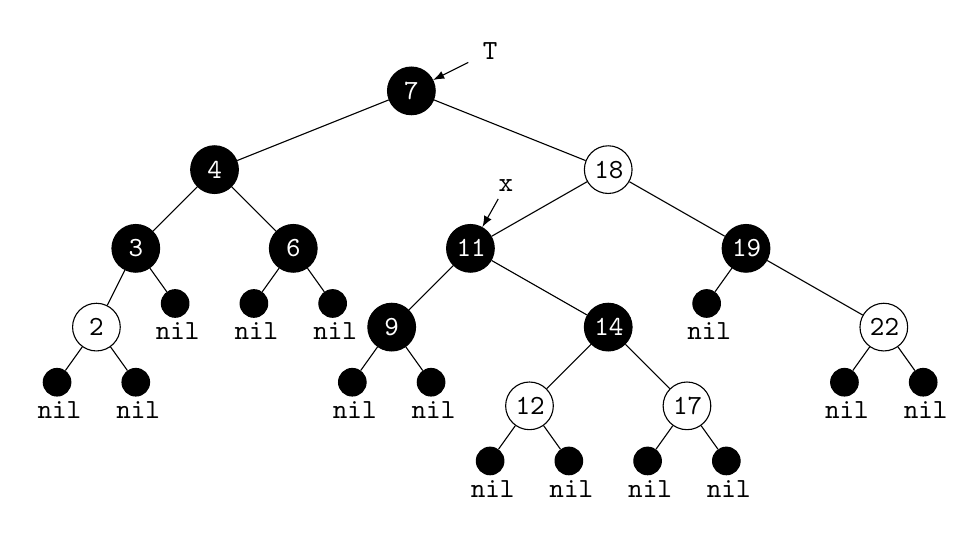
\begin{tikzpicture}
    [edge from parent/.style={draw,-},
    every node/.style={
        text width=1em,
        align=center,
        font=\ttfamily,
        draw,
        circle,
        inner sep=2pt,
        minimum size=8pt},
    level distance=1cm,
    level 1/.style={sibling distance=5cm},
    level 2/.style={sibling distance=2cm},
    level 3/.style={sibling distance=1cm}]
    \node[black] (root) {7}
    child {node[black] {4}
        child {node[black] {3}
            child {node {2}
                child[short] {node[nil] {}}
                child[short] {node[nil] {}}
            }
            child[short] {node[nil] {}}
        }
        child {node[black] {6}
            child[short] {node[nil] {}}
            child[short] {node[nil] {}}
        }
    }
    child {node {18}
        child[sibling distance=3.5cm] {node[black] (axis) {11}
            child[sibling distance=2cm] {node[black] {9}
                child[short] {node[nil] {}}
                child[short] {node[nil] {}}
            }
            child[sibling distance=3.5cm] {node[black] {14}
                child[sibling distance=2cm] {node {12}
                    child[short] {node[nil] {}}
                    child[short] {node[nil] {}}
                }
                child[sibling distance=2cm] {node {17}
                    child[short] {node[nil] {}}
                    child[short] {node[nil] {}}
                }
            }
        }
        child[sibling distance=3.5cm] {node[black] {19}
            child[short] {node[nil] {}}
            child[sibling distance=3.5cm] {node {22}
                child[short] {node[nil] {}}
                child[short] {node[nil] {}}
            }
        }
    };
    \node[draw=none] (T) at (1, .5) {T};
    \draw[-latex] (T) -> (root);

    \node[draw=none, inner sep=0pt] (x) at (1.2, -1.2) {x};
    \draw[-latex] (x) -> (axis);
\end{tikzpicture}
\bigskip

Cet arbre ne vérifie plus la propriété d'arbre bicolore, le nombre de nœuds noirs n'est plus le même sur toutes les branches partant de la racine.

\Q
L'insertion dans un arbre bicolore peut se faire selon le schéma suivant :\\
On insère le nouvel élément dans l'ABR en utilisant la fonction de la question 2 ; on obtient donc un arbre binaire de recherche.\\
Pour que cet arbre vérifie la propriété de bicolore, nous donnons à ce nouveau nœud la couleur rouge. Il devient le nœud courant. Si son père est noir, l'arbre est bicolore et c'est terminé. Sinon, si le frère de ce père est rouge, ce père et son frère deviennent noirs et leur père devient rouge. On recommence avec le père commun. Par contre, si le frère du père du nœud courant est noir, il y a au moins un élément de plus du côté du nœud courant. Dans ce cas, nous plaçons le nœud courant et son père suivant le même type de filiation que le père et le grand-père : le père devient noir et le grand-père rouge puis nous effectuons une rotation dans le sens du père vers son grand père.
\smallskip

On représente ici l'une des quatre situations où une rotation est nécessaire :

\tikzstyle{caption}=[draw=none, fill=none, inner sep=2pt, rectangle]
\begin{center}
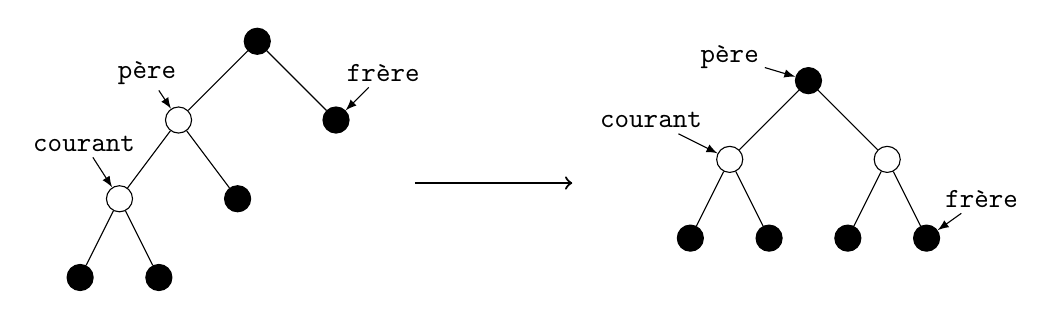
\begin{tikzpicture}[
    level distance=1cm,
    every node/.style={
    font=\ttfamily,
    fill=black,
    circle, draw, fill=black},
    level 1/.style={sibling distance=2cm},
    level 2/.style={sibling distance=1.5cm},
    level 3/.style={sibling distance=1cm}]
    \node {}
    child {node[fill=none] (pere_n) {}
        child {node[fill=none] (courant_n) {}
            child {node {}}
            child {node {}}
        }
        child {node {}}
    }
    child {node (frere_n) {}};

    \node[caption] (frere) at (1.6, -.4) {frère};
    \draw[-latex] (frere) -> (frere_n);

    \node[caption] (pere) at (-1.4, -.4) {père};
    \draw[-latex] (pere) -> (pere_n);

    \node[caption] (courant) at (-2.2, -1.3) {courant};
    \draw[-latex] (courant) -> (courant_n);

    \draw[thick, ->] (2,-1.8) -> (4,-1.8);

    \node[xshift=7cm, yshift=-.5cm] (pere2_n) {}
    child {node[fill=none] (courant2_n) {}
        child[sibling distance=1cm] {node {}}
        child[sibling distance=1cm] {node {}}
    }
    child {node[fill=none] {}
        child[sibling distance=1cm] {node {}}
        child[sibling distance=1cm] {node (frere2_n) {}}
    };

    \node[caption] (frere2) at (9.2, -2) {frère};
    \draw[-latex] (frere2) -> (frere2_n);

    \node[caption] (pere2) at (6, -.2) {père};
    \draw[-latex] (pere2) -> (pere2_n);

    \node[caption] (courant2) at (5, -1) {courant};
    \draw[-latex] (courant2) -> (courant2_n);
\end{tikzpicture}
\end{center}
\medskip

Nous obtenons ainsi les fonctions OCaml suivantes où l'on n'effectue pas de rotation de manière \og explicite \fg{} mais où on utilise une fonction de \textit{pattern-matching} pour gérer les cas où deux nœuds rouges se suivent :

\lstinputlisting[linerange={31-49}]{\SourceFile}

Notons que pour éviter de répéter deux fois la même chose, on pourrait définir une fonction constructeur comme suit :

\lstinputlisting[firstline=51]{\SourceFile}

Nous disposons d'un arbre binaire de recherche dont la profondeur est d'au plus $2\log_2(n+1)$, avec des algorithmes d'insertion et de suppression qui parcourent un nombre donné de fois une branche de l'arborescence. Nous disposons ainsi d'une structure de données où toutes les opérations peuvent se faire en un temps logarithmique suivant la taille de cette base de données.
\bigskip

\Fin
